%%%%%%%%%%%%%%%%%%%%%%%%%%%%%%%%%%%%%%%%%
% Programming/Coding Assignment
% LaTeX Template
%
% This template has been downloaded from:
% http://www.latextemplates.com
%
% Original author:
% Ted Pavlic (http://www.tedpavlic.com)
%
% Note:
% The \lipsum[#] commands throughout this template generate dummy text
% to fill the template out. These commands should all be removed when 
% writing assignment content.
%
% This template uses a Perl script as an example snippet of code, most other
% languages are also usable. Configure them in the "CODE INCLUSION 
% CONFIGURATION" section.
%
%%%%%%%%%%%%%%%%%%%%%%%%%%%%%%%%%%%%%%%%%

%----------------------------------------------------------------------------------------
%	PACKAGES AND OTHER DOCUMENT CONFIGURATIONS
%----------------------------------------------------------------------------------------

\documentclass[a4paper]{article}

\usepackage{fancyhdr} % Required for custom headers
\usepackage{lastpage} % Required to determine the last page for the footer
\usepackage{extramarks} % Required for headers and footers
\usepackage[usenames,dvipsnames]{color} % Required for custom colors
\usepackage{graphicx} % Required to insert images
\usepackage{listings} % Required for insertion of code
\renewcommand*{\lstlistingname}{代码} % change "Listing <ref> to 代码 <ref>
\usepackage{courier} % Required for the courier font
\usepackage{lipsum} % Used for inserting dummy 'Lorem ipsum' text into the template

\usepackage[UTF8]{ctex} % Required for Chinese character
\usepackage{tocloft} % Required for beautiful toc
\usepackage[hidelinks]{hyperref} % Required for clickable toc
\hypersetup{
    colorlinks,
    citecolor=black,
    filecolor=black,
    linkcolor=black,
    urlcolor=black
}
\usepackage[title]{appendix} % Required for appendix
\usepackage{float}
\usepackage{amsmath} % used for \text{} in math formula


% used for beautiful table
\usepackage{booktabs} 
\usepackage[T1]{fontenc}
\usepackage{tabu}
\usepackage{longtable}
\usepackage[table]{xcolor}


% Margins
\topmargin=-0.45in
\evensidemargin=0in
\oddsidemargin=0in
\textwidth=6.5in
\textheight=9.0in
\headsep=0.25in

\linespread{1.1} % Line spacing

% Set up the header and footer
\pagestyle{fancy}
\lhead{\hmwkAuthorName} % Top left header
\chead{\hmwkClass\ (\hmwkClassInstructor\ \hmwkClassTime): \hmwkTitle} % Top center head
\rhead{\firstxmark} % Top right header
\lfoot{\lastxmark} % Bottom left footer
\cfoot{} % Bottom center footer
\rfoot{Page\ \thepage\ of\ \protect\pageref{LastPage}} % Bottom right footer
\renewcommand\headrulewidth{0.4pt} % Size of the header rule
\renewcommand\footrulewidth{0.4pt} % Size of the footer rule

\setlength\parindent{0pt} % Removes all indentation from paragraphs

%----------------------------------------------------------------------------------------
%	CODE INCLUSION CONFIGURATION
%----------------------------------------------------------------------------------------

\definecolor{MyDarkGreen}{rgb}{0.0,0.4,0.0} % This is the color used for comments
\lstloadlanguages{c} % Load Perl syntax for listings, for a list of other languages supported see: ftp://ftp.tex.ac.uk/tex-archive/macros/latex/contrib/listings/listings.pdf
\lstset{language=c, % Use Perl in this example
        frame=single, % Single frame around code
        basicstyle=\small\ttfamily, % Use small true type font
        keywordstyle=[1]\color{Blue}\bf, % Perl functions bold and blue
        keywordstyle=[2]\color{Purple}, % Perl function arguments purple
        keywordstyle=[3]\color{Blue}\underbar, % Custom functions underlined and blue
        identifierstyle=, % Nothing special about identifiers                                         
        commentstyle=\usefont{T1}{pcr}{m}{sl}\color{MyDarkGreen}\small, % Comments small dark green courier font
        stringstyle=\color{Purple}, % Strings are purple
        showstringspaces=false, % Don't put marks in string spaces
        tabsize=4, % 5 spaces per tab
        %
        % Put standard Perl functions not included in the default language here
        % morekeywords={rand},
        morekeywords = [1]{uint16_t, uint32_t, uint8_t, int16_t, int8_t, int32_t}
        %
        % Put Perl function parameters here
        morekeywords=[2]{on, off, interp, __attribute__},
        %
        % Put user defined functions here
        morekeywords=[3]{test},
       	%
        morecomment=[l][\color{Blue}]{...}, % Line continuation (...) like blue comment
        numbers=left, % Line numbers on left
        firstnumber=1, % Line numbers start with line 1
        numberstyle=\tiny\color{Blue}, % Line numbers are blue and small
        stepnumber=2, % Line numbers go in steps of 5,
        firstnumber=1
}

% define C style
\definecolor{main-color}{rgb}{0.6627, 0.7176, 0.7764}
\definecolor{back-color}{rgb}{0.1686, 0.1686, 0.1686}
\definecolor{string-color}{rgb}{0.3333, 0.5254, 0.345}
\definecolor{key-color}{rgb}{0.8, 0.47, 0.196}
\lstdefinestyle{mystyle}
{
    language = C++,
    basicstyle = {\small\ttfamily},
    stringstyle = {\color{Mahogany}},
    keywordstyle = {\color{blue}},
    keywordstyle = [2]{\color{Mahogany}},
    keywordstyle = [3]{\color{blue}},
    keywordstyle = [4]{\color{blue}},
    otherkeywords = {__attribute__,<<,>>,++},
    morekeywords = [2]{__attribute__},
    morekeywords = [3]{<<, >>},
    morekeywords = [4]{++, uint16_t, uint32_t, uint8_t, \#define},
}


% Creates a new command to include a perl script, the first parameter is the filename of the script (without .pl), the second parameter is the caption

\newcommand{\shfilescript}[3]{
\begin{itemize}
\item[]\lstinputlisting[caption=#2, label=lst:#1, language=sh]{#3}
\end{itemize}
}
\newcommand{\shscript}[3]{
\begin{itemize}
\item[]\begin{lstlisting}[label=lst:#1, caption=#2] #3 \end{lstlisting}
\end{itemize}
}

%----------------------------------------------------------------------------------------
%	DOCUMENT STRUCTURE COMMANDS
%	Skip this unless you know what you're doing
%----------------------------------------------------------------------------------------

% Header and footer for when a page split occurs within a problem environment
\newcommand{\enterProblemHeader}[1]{
\nobreak\extramarks{#1}{#1 见下页\ldots}\nobreak{} 
\nobreak\extramarks{接上页}{#1 见下页\ldots}\nobreak{}
}

% Header and footer for when a page split occurs between problem environments
\newcommand{\exitProblemHeader}[1]{
\nobreak\extramarks{接上页}{#1 见下页\ldots}\nobreak{}
\nobreak\extramarks{#1}{}\nobreak{}
}
% TODO:code here enable the number before section, but it disable the numbering of problems
%\setcounter{secnumdepth}{0} % Removes default section numbers
\newcounter{homeworkProblemCounter} % Creates a counter to keep track of the number of problems

\newcommand{\homeworkProblemName}{}

\newenvironment{homeworkProblem}[1][Problem \arabic{homeworkProblemCounter}]{ % Makes a new environment called homeworkProblem which takes 1 argument (custom name) but the default is "Problem #"
\stepcounter{homeworkProblemCounter} % Increase counter for number of problems
\renewcommand{\homeworkProblemName}{#1} % Assign \homeworkProblemName the name of the problem
\section{\homeworkProblemName} % Make a section in the document with the custom problem count
\enterProblemHeader{\homeworkProblemName} % Header and footer within the environment
}{
\exitProblemHeader{\homeworkProblemName} % Header and footer after the environment
}

\newcommand{\problemAnswer}[1]{ % Defines the problem answer command with the content as the only argument
\noindent\framebox[\columnwidth][c]{\begin{minipage}{0.98\columnwidth}#1\end{minipage}} % Makes the box around the problem answer and puts the content inside
}

\newcommand{\homeworkSectionName}{}
\newenvironment{homeworkSection}[1]{ % New environment for sections within homework problems, takes 1 argument - the name of the section
\renewcommand{\homeworkSectionName}{#1} % Assign \homeworkSectionName to the name of the section from the environment argument
\subsection{\homeworkSectionName} % Make a subsection with the custom name of the subsection
\enterProblemHeader{\homeworkProblemName\ [\homeworkSectionName]} % Header and footer within the environment
}{
\enterProblemHeader{\homeworkProblemName} % Header and footer after the environment
}


\newcommand{\codev}[1]{\textsf{#1}}
%----------------------------------------------------------------------------------------
%	NAME AND CLASS SECTION
%----------------------------------------------------------------------------------------

% table color
\definecolor{tableHeader}{RGB}{245, 245, 245}
\definecolor{tableLineOne}{RGB}{245, 245, 245}
\definecolor{tableLineTwo}{RGB}{224, 224, 224}
\newcommand{\tableHeaderStyle}{
    \rowfont{\leavevmode\color{white}\bfseries}
    \rowcolor{tableHeader}
}

%----------------------------------------------------------------------------------------

\newcommand{\hmwkTitle}{操作系统原理实验\ \#5} % Assignment title
\newcommand{\hmwkDueDate}{Friday,\ April\ 13,\ 2018} % Due date
\newcommand{\hmwkClass}{16级计科\ 7班} % Course/class
\newcommand{\hmwkClassTime}{周一9-10节} % Class/lecture time
\newcommand{\hmwkClassInstructor}{凌应标} % Teacher/lecturer
\newcommand{\hmwkAuthorName}{颜彬} % Your name
\newcommand{\hmwkAuthorId}{16337269} % Your id 

%----------------------------------------------------------------------------------------
%	TITLE PAGE
%----------------------------------------------------------------------------------------

\usepackage{titling}

\title{
\vspace{2in}
\textmd{\textbf{\hmwkClass:\ \hmwkTitle}}\\
\normalsize\vspace{0.1in}\small{Due\ on\ \hmwkDueDate}\\
\vspace{0.1in}\large{\textit{\hmwkClassInstructor\ \hmwkClassTime}}
\vspace{3in}
}

\author{\textbf{\LARGE{\hmwkAuthorName}} \\ \\ \textbf{\LARGE{\hmwkAuthorId}}}
\date{} % Insert date here if you want it to appear below your name
%----------------------------------------------------------------------------------------

\begin{document}
% \begin{titlingpage} % This is for ignore page number in first page. package titling

\maketitle

%----------------------------------------------------------------------------------------
%	TABLE OF CONTENTS
%----------------------------------------------------------------------------------------

% \setcounter{tocdepth}{2} % Uncomment this line if you don't want subsections listed in the ToC
% set depth in toc

% \renewcommand{\cftsecleader}{\cftdotfill{\cftdotsep}} % used for dots between <section> and <page>

\renewcommand{\contentsname}{Content} % force the word to be "content
\newpage
\tableofcontents
\addtocontents{toc}{~\hfill\textbf{Page}\par}
\newpage

% below are document body


% To have just one problem per page, simply put a \clearpage after each problem
\section{实验目的}
掌握PC微机的实模式硬件中断系统原理和中断服务程序设计方式,实现对时钟、
键盘/鼠标等硬件中断的简单服务处理程序编程和调试,让你的原型操作系统
在运行以前已有的用户程序时,能对异步事件正确地捕捉和响应。\\

掌握操作系统的系统调用原理,实现原型操作系统中的系统调用框架,提供若干
简单功能的系统调用。 \\

学习掌握C语言库的实际方法,为自己的原型操作系统配套一个C程序开发环境,
实现用自建的C语言开发简单的输入/输出的用户程序,展示封装的系统调用。
\section{实验方案}
    \subsubsection{中断调用原理}
    在实模式下,内存0x0000起始处维护着一张中断服务程序入口的表。每个
    表项站4字节,共同代表服务程序的入口地址。其中的低16位代表代码段
    地址,高16位代表段内偏移地址。\\
    
    当调用中断时,中断号代表着服务程序地址在地址表中的索引。所以当
    执行int $id$时,会将$0x0000 : id \times 4$起始的32 bits
    作为入口地址。一般寄存器ah中的值会作为中断的``功能号''。其他寄存器
    的值依据文档,相应地作为参数或作为返回值。\\
    
    当实模式下触发中断时,会首先将FLAGS寄存器压入栈中(32位模式下
    是EFLAGS),随后压入
    cs:ip,并根据地址表中的信息,跳转到相应地址。在中断返回时,要
    首先向硬件端口输出相应参数,告知中断处理硬件中断完成。随后,iret
    指令将把FLAGS和cs:ip出栈,并跳转回相应的用户程序地址。\\
    
    这些中断调用的原理就给了自定义中断的可能。用户只需修改中断地址表,
    并按照中断的行为书写自己的代码,就能实现自己的中断。 
    \subsubsection{软硬中断简介}
    软件和硬件都能引发中断。其中软件中断又称为系统调用。其与调用一个函数
    (在程序员可见角度)类似,有输入的参数和相应的返回值。程序员在系统
    调用前应手动保存需要保存的寄存器,并能预计到中断会修改相应寄存器的值。
    系统调用都是不可屏蔽的。\\ 
    
    硬件中断有可屏蔽和不可屏蔽两种。其中时钟中断(watchdog)是
    不可屏蔽中断。由于硬件中断可以发生在任何一个时间点,所以硬件中断
    应能保证绝对不修改任何寄存器的值。即硬件中断对程序员是透明的。
    \subsubsection{用户自定义中断}
    用户自定义中断可以采用如下的方式。首先查阅中断地址表,找到未被
    占用的中断号(例如本项目使用的0x2B号)。将地址表的相应表项修改
    用户自定义的地址。则当中断发生时,程序控制流可以到达用户自定义地址。\\
    
    标准的中断实现中,用户自定义中断应该提取ah作为功能号,建立中断自己的
    功能地址表,根据ah的值在功能地址表中提取相应功能的中断入口地址,并跳转
    到该地址。\\
    
    中断返回时,要保证将栈退到``刚进入中断''时的状态,向硬件端口传送一些
    数据,并用iret指令返回。
    \subsection{实验环境}
    \subsubsection{系统与虚拟机}
    \begin{itemize} \item 操作系统 \\ 
        本实验在Linux下完成。采用Ubuntu 16.04
        \item 虚拟机\\
        bochs.它是一款开源且跨平台的 IA-32 模拟器。
    \end{itemize}
    \subsubsection{相关工具、指令}
        \begin{itemize}
            \item 汇编器\\ 
            NASM. NASM是一个轻量级的、模块化的 80x86 和 x86-64 汇编器。它的语法与
            Intel 原语法十分相似,但更加简洁和易读。它对宏有十分强大的支持。
            \item 编译器\\
            GCC. GNU/GCC 是开源的C语言编译器。其产生的伪16位代码可以与NASM结合,混编生成伪16位程序。
            \item 镜像文件产生工具\\ 
            bximage. 该命令允许生成指定大小的软件镜像。
            \item 二进制写入命令\\ 
            dd. dd 允许指定源文件和目标文件,将源文件的二进制比特写入目标文件中的指定位置。
            \item 二进制文件查看命令\\ 
            xxd. xxd 允许将二进制文件中的内容按地址顺序依次输出,可读性强
            \item 反汇编器\\
            objdump. objump可以查看目标文件和二进制文件的反汇编代码,还能指令intel或at\&t格式显示。
            \item 代码生成脚本\\
            makefile. makefile脚本具有强大的功能,其可以识别文件依赖关系,自动构筑文件,自动执行shell脚本等。
        \end{itemize}
 
\section{实验过程}
    \subsubsection{GCC语言拓展的运用}\label{subsec:asm}
    为了简化代码的书写,本项目进一步地使用了GCC的语言拓展,\_\_asm\_\_语法。代码\ref{lst:asm_ext}举出了两个
    比较有说明性的道理,列举其用法。内嵌汇编的初衷是,若C语言不得不调用汇编,而汇编语句又很短(10行以内),为了汇编
    而新建一个文件并编译链接显得很麻烦。内嵌汇编可以做到``细粒度''的C与汇编交互功能。\\
    
    volatile语句的作用是``禁止GCC优化(删除)掉汇编语句''。由于GCC在编译时无法解析汇编的内容,汇编的内容是在C
    语言代码完全编译后,再由内置汇编器解释的。故GCC无法在编译期确定内嵌的汇编代码是否有副作用。若GCC(错误地)认为
    这些汇编代码没有副作用,会把代码完全优化(删除)掉。volatile可以禁止这种优化。\\
    
    整个拓展语法为\_\_asm\_\_ volatile ( assembly : output : input : clobber );\\
    
    其中assembly为字符串表示的汇编代码。以回车结尾以分隔汇编代码。output显式地指明了汇编代码会``输出''到C变量,即
    汇编代码会修改某个C变量的值。input显示地指明了汇编代码会从C语言``输入''值,即把C的某个变量赋给寄存器。clobber
    显式地指明了汇编语句会修改到哪些内容(如标志寄存器,内存等)。如果不指明,C语言会(为了速度)而不刷新缓存,导致
    汇编语句的修改没有更新到C语言环境中。\\
    
    代码\ref{lst:asm_ext}中,``c'', ``D''分别代表寄存器CX和DX,``CC''表示标志寄存器,其他标志可从字面意思弄懂。
    这些标志与架构密切相关,可以从GCC官网的ASM语言拓展查到详细的使用手册。\\
    
    代码\ref{lst:asm_ext}的两个函数中,第一个函数通过中断的方式在屏幕的某个特定的位置显示字符。C语言对它做了便利
    的封装。第二个函数用于得到光标位置,并自动导出到cursor\_pos中。
    \begin{figure}[!htb]
    \begin{itemize}
    \item[] \begin{lstlisting}[language=C, label=lst:asm_ext, caption=GCC内嵌汇编拓展语法详解]
static inline int16_t _draw_char(char ch, int offset, uint8_t style) {
    uint16_t written_data = ch | (style << 8);
    __asm__ volatile (
        "movb $1, %%ah\n"
        "int $0x2B\n"
        : /* no output */
        : "c"(written_data), "D"(offset)
        : "cc", "ax", "memory"
    );
    return 1;
}
static inline uint16_t get_cursor(){
    uint16_t cursor_pos;
    __asm__ volatile(
        "pushw %%ax\n"
        "pushw %%bx\n"
        "movb $0x03, %%ah\n"
        "movb $0, %%bh\n"
        "int $0x10\n"
        "popw %%bx\n"
        "popw %%ax\n"
        : "=d"(cursor_pos)
        : /* no input */
        : "cc", "cx"
    );
    return cursor_pos;
}
    \end{lstlisting}
    \end{itemize}
    \end{figure}
    \subsection{修改时钟中断}
    本步骤的重点在于,保证时钟中断结束后不修改\textbf{任何}寄存器的值,且进入时钟中断的时立即将段寄存器初始化到正确的
    状态.\\
    
    由于时钟中断可以发生在代码执行的任何一个时刻,用户程序在执行到任何一个状态时,都有可能被突然间中断。如果时钟中断没有
    保存(哪怕一个)寄存器的值,当中断返回时,用户程序会直接崩溃。更可怕的是,有可能用户程序不立即崩溃,带着错误的状态继续
    执行下去,错误像滚雪球般地越积越多。当程序错误地退出时,很难定位到BUG的具体发生位置。\\
    
    更需要注意的是,在时钟中断进入后,要尽快地将ds的值设置为cs的值。虽然本项目使用平坦模型(flatten model),
    段寄存器的值都是0,但是由于时钟中断可以发生在任何时候(哪怕当前正在运行另外一个中断)。而另外的中断(例如int 16H)
    的代码中很可能临时地修改段寄存器。在时钟中断突然来临后,ds的值将是错误的值。这同样会导致程序的异常出现。\\
    
    代码\ref{lst:clock_int}展示了自定义时钟中断的实现。假设代码已经成功地将中断向量表地址修改为timeOut汇编函数的
    首地址。timeOut后,程序会先保存一些寄存器的值,将ds同步为cs,随后使用call指令调用C的真正的处理函数。当从C函数中
    返回后,恢复相关寄存器,随后跳转到原时钟中断(0F000H:0FEA5H)的地址。由于不清楚原时钟中断做了什么,所以最好在程序
    最后跳转回原中断,让它完成它想完成的事情。
    \begin{figure}[!bht]
    \begin{itemize}
    \item[] \begin{lstlisting}[language={[x86masm]Assembler}, label=lst:clock_int, caption=自定义时钟中断的部分代码]
timeOut:

    pusha
    push gs
    push ds
    push es

    mov ax, cs 
    mov ds, ax 
    mov es, ax 

    push cs 
    call timeout ; timeout is a C function

    pop es
    pop ds
    pop gs
    popa

    jmp 0F000H:0FEA5H ; 为了展示目的,这里采用硬编码的方式
    \end{lstlisting}
    \end{itemize}
    \end{figure}
    \subsection{修改键盘中断}
    键盘中断的实现和时钟中断十分类似。首先修改中断向量表,保证中断发生时控制权能到达用户自定义程序。只要保证能恢复
    到中断前的状态,程序一般就能正确运行。\\
    
    本个实现的小技巧是,采用pushf 和 call far的方式先调用旧键盘中断处理程序。由于旧中断处理程序的最后一条指令必为iret,
    刚好可以把pushf 和call far中压栈的内容正确地恢复到原有的寄存器中。随后自定义中断服务程序再通过一个iret把栈完全复原。
    \subsection{安装用户自定义中断}
    为了让用户自定义中断的行为和系统自带的中断保持类似,自定义中断也采用ah作为功能号标志。具体实现如代码\ref{lst:custom_int}所示。\\

    global\_custom\_int\_install函数安装用户自定义中断,把2BH号中断链接到custom\_int\_hanlder函数中。该函数是个
    中断处理函数,它负责解析功能号(ah)的值,在一个向量表中查询服务程序的地址,并将控制权移交给服务程序。值得注意的是,
    所有的服务程序都通过retf的方式先返回到custom\_int\_handler,由其统一地使用iret结束中断。也就是custom\_int\_handler
    是一个统一的入口和出口,做了封装和``分发处理''。\\
    
    custom\_int\_table地址表。功能号ah代表着地址在表中的位置。本项目定义了三个简单的中断程序。第一个叫testcase,它做了
    若干入栈和出栈操作。它用来检测``从中断安装到中断执行''的过程中,栈是否正确地返回了。\_int\_draw\_char是重写的底层输出
    函数。所有的IO函数几乎都依赖于这一中断调用。见//TODO:\_draw\_char
    的介绍。
    \_int\_draw\_my\_info中断会在程序的特定位置显示3-D的学号。视觉效果较好。
    
    \begin{figure}[!h]
    \begin{itemize}
    \item[] \begin{lstlisting}[language={[x86masm]Assembler}, label=lst:custom_int, caption=用户自定义中断的实现]
global_custom_int_install:
    push ds
    mov ax, 0
    mov ds, ax

    mov word [ds:2BH * 4], custom_int_handler
    mov word [ds:2BH * 4 + 2], cs

    pop ds
    retl
custom_int_handler:
    ; ah=01H: _draw_char
    push bx
    push ax
    push dx 

    mov dl, 4
    mov al, ah
    xor ah, ah
    mul dl
    add ax, custom_int_table
    mov bx, ax

    pop dx
    pop ax

    call far [bx]

    pop bx
    iret

testcase:
    ...

    retf
_int_draw_char:
    ...

    retf

_int_draw_my_info:
    ...

    retf
custom_int_table:
    dw testcase
    dw 0x0000
    dw _int_draw_char
    dw 0x0000
    dw _int_draw_my_info
    dw 0x0000  
    \end{lstlisting}
    \end{itemize}
    \end{figure}
\section{实验结果}
\subsection{终端界面}
图\ref{fig:terminal}展示了终端界面的外观。//TODO:由于四周围的边框
需要有闪动的字符,所以终端的所有提示信息都应自动地为边框腾出空间。为了完成
这个效果,本项目结合了滚屏中断和光标设置中断,实现了一个特殊的字符输出中断,
原本写好的IO程序可以不加修改,只修改他们底层最终依赖的中断,即可自动地为
边框腾出空间。\\

图\ref{fig:terminal}还同时展示了改进版的ls指令。该指令会用对齐的
方式输出根目录的所有文件,文件的大小以及文件所在的首扇区。对齐的输出
使用了新增的printf定宽输出功能。见//TODO:\\

文件系统其实还实现了输出文件所有簇编号这一功能。只是由于内核程序太大,所
占的簇数太多,导致输出的画面显得混乱。所以在这个版本中我把这个功能砍掉了。
但我保留了一张截图,如\ref{fig:fs_long_ls.png}所示。
\begin{figure}
    \begin{center}
    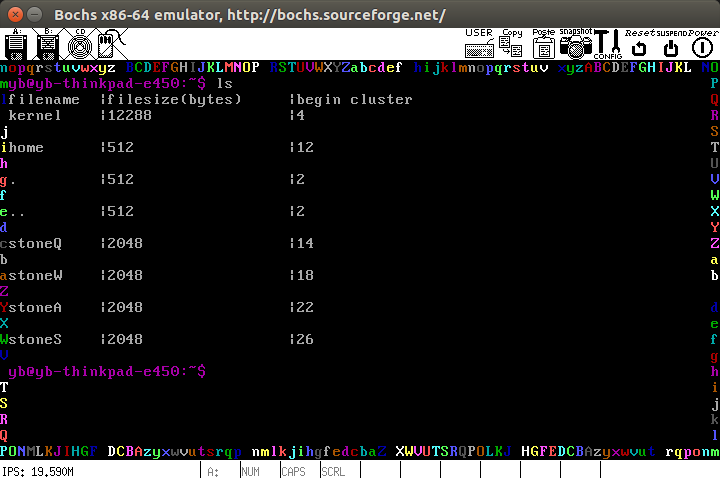
\includegraphics[scale=0.5]{assets/terminal.png}
    \caption{带运动边框的终端界面\label{fig:terminal}} 
    \end{center} 
\end{figure} 

\begin{figure}
    \begin{center}
    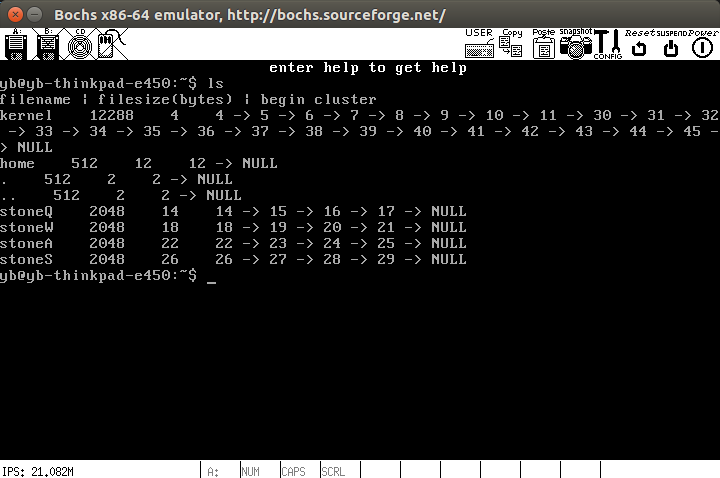
\includegraphics[scale=0.5]{assets/fs_long_ls.png}
    \caption{带有文件所有扇区列表的ls指令\label{fig:ls}} 
    \end{center} 
\end{figure} 
\subsection{用户程序}
图\ref{fig:user}实现了带按键反馈的用户程序。在进入用户程序时,安装
自定义中断,键盘对每次按下都会输出 ``OUCH!'',而在离开用户程序后,中断
复原,不再对键盘按下响应``OUCH!''。\\

\begin{figure}
    \begin{center}
    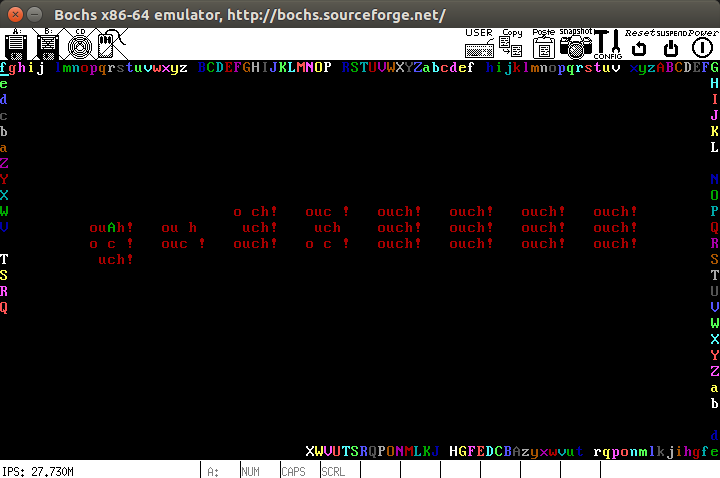
\includegraphics[scale=0.5]{assets/user.png}
    \caption{带按键反馈的用户程序\label{fig:user}} 
    \end{center} 
\end{figure} 

\subsection{特色中断}
本实现实现了特色中断,可以以3D的形式输出本人的学号。如图\ref{fig:3_D_id}
所示。

\begin{figure}
    \begin{center}
    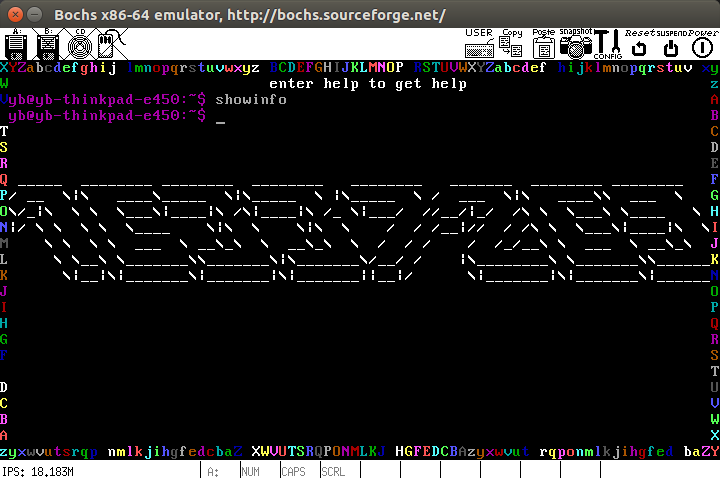
\includegraphics[scale=0.5]{assets/16337269.png}
    \caption{特色中断:个人学号的3D显示\label{fig:3_D_id}} 
    \end{center} 
\end{figure} 

\section{实验总结}
    \subsection{亮点介绍}
    \subsubsection{极其详尽的文档}
    本次项目为所有文件添加了足够的注释,并自动生成了说明文档。
    说明文档可以见网页\\ 

    \url{https://yanb25.github.io/OperatingSystem/files.html}。(可点击) \\

    其上极其详细地为几乎所有函数增加说明,列举了函数间的依赖关系以及
    调用方法等。\\
    
    同时,本项目中附属的项目文档pdf文件也由代码和注释自动生成。
    \subsubsection{ASM拓展语法}
    本实验在上个实验的基础上,更深入地使用了GCC的ASM语言拓展。为
    C和汇编的交互带来了更大的便利。见\ref{subsec:asm}节。
    \subsubsection{格式化ls输出}
    本实验实现了格式化的ls输出,在输出文件名的同时,格式化地输出
    文件大小和文件首簇位置。本实验还实现了函数,可以将文件的所有簇
    按序输出。见图\ref{fig:fs_long_ls.png}和图\ref{fig:terminal}。其他寄存器
    \subsubsection{光标滚屏自主控制}
    为了完成终端中闪烁的边框,本项目将IO函数的一个底层中断重写了一遍。并
    结合了光标控制和自动滚屏。见//TODO:所示。

    \subsection{更新细节}
    \subsubsection{printf进一步完善}
    实现了定宽输出的功能。即支持$ printf("\%4d", 1) $ 功能,
    在输出的1前输出3个空格。//TODO:
    \\
    同时,所有的IO函数重构成返回int16\_t类型,代表他们输出到屏幕的
    字符数。这为格式化输出提供了巨大的帮助。
    \subsubsection{目录树结构变更}
    将C程序库进一步细分,分成了utilities.h, stdio.h, ctype.h, mystring.h 
    等基本库。utilities.h负责内核所需的最基本的操作,例如扇区读写和
    光标控制等。其他头文件作用类似与ANSI C的实现。
    \subsection{心得体会}
 
    \subsection{BUG汇总}
    \subsubsection{扇区加载错误}
    首先是发生了扇区加载不足的状况。操作系统内核共10个展区长度,但在最开始的实现中
    只//TODO:
\begin{appendices}
\section{参考文献} \label{sec:reference}
sasadf
\begin{enumerate}
    \item https://blog.csdn.net/longintchar/article/details/50602851 \\
    16位和32位汇编指令的不同(尤其是push指令)
    \item https://www.ibiblio.org/gferg/ldp/GCC-Inline-Assembly-HOWTO.html\#s1 \\
    GCC 内嵌汇编的书写。
    \item http://blog.51cto.com/dengqi/1349327
    FAT32文件系统讲解
    \item https://blog.csdn.net/yeruby/article/details/41978199
    FAT16文件系统讲解
  \end{enumerate}
\section{其他代码} \label{sec:otherCode}
\end{appendices}
\end{document}